\section{Análise da Correlação entre as Taxas de Upload e Download para os Horários com o Maior Valor de Tráfego}

Nesta seção, foi analisada a relação entre as taxas de upload e download para os horários de maior tráfego identificados previamente. Para isso, foram calculados os coeficientes de correlação amostral e gerados gráficos de dispersão (\textit{scatter plots}) comparando as taxas de upload e download para os dispositivos Smart TV e Chromecast.

\subsection{Cálculo do Coeficiente de Correlação}

O coeficiente de correlação de Pearson foi calculado para cada dispositivo, utilizando o método \texttt{corr} da biblioteca \texttt{pandas} do Python. O coeficiente de correlação varia de -1 a 1, onde valores próximos de 1 indicam uma correlação positiva forte, valores próximos de -1 indicam uma correlação negativa forte e valores próximos de 0 indicam ausência de correlação.

considerando os datasets correspondentes aos horários selecionados:
\begin{itemize}
    \item \textbf{Smart TV:} Comparação entre o Dataset 1 (Upload) e o Dataset 2 (Download).
    \item \textbf{Chromecast:} Comparação entre o Dataset 3 (Upload) e o Dataset 4 (Download).
\end{itemize}

Os valores dos coeficientes de correlação para cada dispositivo são apresentados na Tabela~\ref{tab:coeficientes_correlacao}.

\begin{table}[H]
    \centering
    \caption{Coeficientes de correlação amostral entre as taxas de upload e download.}
    \label{tab:coeficientes_correlacao}
    \begin{tabular}{|c|c|}
        \hline
        \textbf{Dispositivo} & \textbf{Coeficiente de Correlação} \\ \hline
        Smart TV & 0.9156 \\ \hline
        Chromecast & 0.2248 \\ \hline
    \end{tabular}
\end{table}

\subsection{Gráficos de Dispersão}

Os gráficos de dispersão foram gerados para ilustrar a relação entre as taxas de upload e download para os dois dispositivos. Esses gráficos estão apresentados na Figura~\ref{fig:scatter_plot}.

\begin{figure}[H]
    \centering
    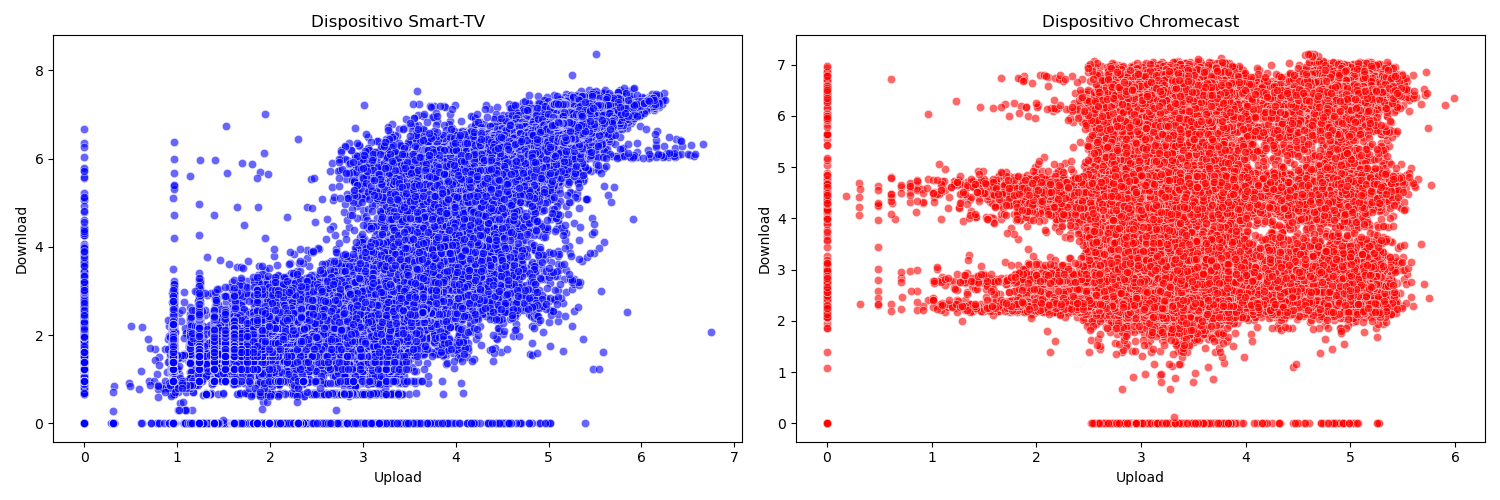
\includegraphics[width=0.8\textwidth]{../correlação/scatter_plot.png}
    \caption{Gráficos de dispersão entre as taxas de upload e download para os dispositivos Smart TV e Chromecast.}
    \label{fig:scatter_plot}
\end{figure}

\subsection{Análise dos Resultados}

Os resultados apresentados demonstram padrões distintos na relação entre as taxas de upload e download para os dispositivos Smart TV e Chromecast. 

Para a Smart TV, o coeficiente de correlação de 0.9156 indica uma forte relação positiva entre as taxas de upload e download. Esse comportamento é evidenciado no gráfico de dispersão (Figura~\ref{fig:scatter_plot}), onde os pontos formam um padrão alinhado, sugerindo que aumentos em uma taxa estão fortemente associados a aumentos na outra. A concentração dos pontos reflete também a homogeneidade dos dados durante o horário analisado, reforçando a sincronização entre os \textit{datasets} 1 e 2, uma vez que os horários de maior tráfego coincidem (20h para ambos).

Por outro lado, o Chromecast apresentou um coeficiente de correlação de 0.2248, indicando uma relação positiva fraca entre as taxas de upload e download. No gráfico de dispersão, os pontos estão significativamente mais espalhados, sugerindo uma menor dependência entre as duas taxas. Esse comportamento pode ser atribuído à falta de sincronização entre os horários analisados nos \textit{datasets} 3 e 4 (22 e 23h, respectivamente), o que resulta em padrões de tráfego menos alinhados.





